\documentclass[a4paper, twoside]{report}
\usepackage[margin=0.5in]{geometry}
\usepackage{amsmath}
\usepackage{amsfonts}
\usepackage{amssymb}
\usepackage{amsthm}
\usepackage{graphicx}
\usepackage{physics}
\usepackage{tikz}
\usepackage{mathrsfs}
\usepackage{pgfplots}
\usepgfplotslibrary{polar}
\usepgfplotslibrary{fillbetween}
\pgfplotsset{compat=1.18}
\usetikzlibrary{arrows,patterns, backgrounds, calc,fadings,shadows.blur, shapes}
\theoremstyle{plain}
\usepackage[most]{tcolorbox}
\usepackage{physunits}
\usepackage{float}
\usepackage[stable]{footmisc}
\usepackage{xcolor}
\usepackage{wrapfig}
\usepackage{microtype}
\usepackage{thmtools}
\usepackage[framemethod=TikZ]{mdframed}
\usepackage{steinmetz}
\usepackage{adjustbox}
\usepackage{listings}
\usepackage[version=4]{mhchem}
\newcommand{\floor}[1]{\lfloor #1 \rfloor}
\newcommand*{\Perm}[2]{{}^{#1}\!P_{#2}}%
\newcommand*{\Comb}[2]{{}^{#1}C_{#2}}%
\mdfsetup{skipabove=1em,skipbelow=0em}
\tcbuselibrary{xparse}
\usepackage[font=small,labelfont=bf,margin=\parindent,tableposition=top]{caption}
\newenvironment{solution}
{\renewcommand\qedsymbol{$\blacksquare$}\begin{proof}[Solution]}
	{\end{proof}}


\declaretheoremstyle[
headfont=\bfseries\sffamily\color{blue!70!black}, bodyfont=\normalfont,
mdframed={
	linewidth=2pt,
	rightline=false, topline=false, bottomline=false,
	linecolor=blue, backgroundcolor=blue!5,
}
]{thmbluebox}
\declaretheorem[style=thmbluebox, numbered=no, name=Example]{eg}


\declaretheoremstyle[
headfont=\bfseries\sffamily\color{blue!70!black}, bodyfont=\normalfont,
numbered=no,
mdframed={
	linewidth=2pt,
	rightline=false, topline=false, bottomline=false,
	linecolor=blue, backgroundcolor=blue!1,
},
]{thmexplanationbox}
\declaretheorem[style=thmexplanationbox, name=Solution]{tmpexplanation}
\newenvironment{explanation}[1][]{\vspace{-10pt}\begin{tmpexplanation}}{\end{tmpexplanation}}


\declaretheoremstyle[
headfont=\bfseries\sffamily\color{red!70!black}, bodyfont=\normalfont,
mdframed={
	linewidth=2pt,
	rightline=false, topline=false, bottomline=false,
	linecolor=red, backgroundcolor=red!5,
}
]{thmredbox}
\declaretheorem[style=thmredbox, name=Theorem]{theorem}

\declaretheoremstyle[
headfont=\bfseries\sffamily\color{red!70!black}, bodyfont=\normalfont,
numbered=no,
mdframed={
	linewidth=2pt,
	rightline=false, topline=false, bottomline=false,
	linecolor=red, backgroundcolor=red!2,
},
qed=\qedsymbol
]{thmproofbox}
\declaretheorem[style=thmproofbox, name=Proof]{replacementproof}
\renewenvironment{proof}[1][\proofname]{\vspace{-10pt}\begin{replacementproof}}{\end{replacementproof}}

\declaretheoremstyle[
headfont=\bfseries\sffamily\color{brown!70!black}, bodyfont=\normalfont,
mdframed={
	linewidth=2pt,
	rightline=false, topline=false, bottomline=false,
	linecolor=brown, backgroundcolor=brown!5,
}
]{thmbrownbox}
\declaretheorem[style=thmbrownbox, numbered=no, name=Question]{asign}

\declaretheoremstyle[
headfont=\bfseries\sffamily\color{brown!70!black}, bodyfont=\normalfont,
numbered=no,
mdframed={
	linewidth=2pt,
	rightline=false, topline=false, bottomline=false,
	linecolor=brown, backgroundcolor=brown!1,
},
]{thmansbox}
\declaretheorem[style=thmansbox, name=Answer]{thmbrown}
\newenvironment{anse}[1][]{\vspace{-10pt}\begin{thmbrown}}{\end{thmbrown}}

\tikzset {_uty0p60aj/.code = {\pgfsetadditionalshadetransform{ \pgftransformshift{\pgfpoint{0 bp } { 0 bp }  }  \pgftransformrotate{-270 }  \pgftransformscale{2 }  }}}
\pgfdeclarehorizontalshading{_zo7gli6ny}{150bp}{rgb(0bp)=(0.6,0.85,1);
rgb(53.66071428571429bp)=(0.6,0.85,1);
rgb(61.60714285714286bp)=(0,0.5,0.5);
rgb(100bp)=(0,0.5,0.5)}
\tikzset{every picture/.style={line width=0.75pt}} %set default line width to 0.75pt 

\usepackage[hidelinks]{hyperref}

\begin{document}
	\begin{titlepage}
		\begin{center}
			\Huge{Fundamentals of Electrical Engineering (FCEE0106)}\\
			Srijan Mahajan (2023UCM2326)\\
			Prof. Vineet Kumar
		\end{center}
	\end{titlepage}
	\tableofcontents
	\newpage
	
	\chapter{Basics Of Measurements}
	We can define the following for measurements,
	\section{Accuracy}
	It is the degree of closeness with which the instrument reading approaches the true value of the quantity to be measured. It can be expressed as,
	\subsection{Percentage of Full Scale Reading}
	In case of instruments having uniform scale, the accuracy can be expressed as percentage of full scale reading.
	\subsection{Percentage of True Value}
	This is the best method of specifying the accuracy. It is to be specified in terms of the true value of quantity being measured.
	\subsection{Point Accuracy}
	Such an accuracy is specified at only one particular point of scale.
	\subsection{Percentage of Scale Span}
	\section{Tolerance}
	Tolerance is a term that is closely related to accuracy and defines the maximum error that is to be expected in some value. It is commonly used to describe the maximum deviation of a manufactured component from some specified value.
	\section{Precision}
	It is the measure of consistency or repeatability of measurements. Precision is a term that describes an instrument’s degree of freedom from random errors.
	\[\text{Precision}=\frac{\text{measured range}}{\text{standard deviation}}\]
	\section{Reliability}
	It refers to how consistently a method measures something. If the same method can be consistently used to achieve the same result under the same circumstances, then the measurement is said to be reliable.
	\section{Repeatability}
	The system design which produces the same high quality product, consistently is said to have high repeatability.
	\section{Resolution}
	The resolution or discrimination of any instrument is the smallest change in the input signal (quantity under measurement) which can be detected by the instrument.
	\section{Noise}
	It is any signal that does not convey any useful information.
	\section{Range}
	It the difference between the maximum and minimum values which can be measured by the instrument.
	\section{Static Sensitivity}
	The ratio of change in output($\Delta A_{\text{out}}$) of an instrument for a given change in the input($\Delta A_{\text{in}}$ that is to be measured is called sensitivity, S.
	\[S=\frac{\Delta A_{\text{out}}}{\Delta A_{\text{in}}}\]
	$\frac{1}{S}$ is called the deflection factor.
	\chapter{Direct-Current Circuits}
	\section{Ohm's Law}
	Ohm's Law states that the potential difference across any two points of the conductor, will be proportional to the current flowing through it.
	\[\begin{split}
		V&\propto I\\
		\therefore V=RI
	\end{split}\]
	\subsection{Star-Delta Transformations}
	\begin{figure}[H]
		\centering
		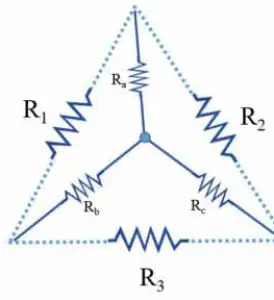
\includegraphics[scale=0.5]{Star-Delta_img.png}
	\end{figure}
	Here, we can convert Star to Delta and vice-versa to make circuit easier to solve,
	\[R_1=R_a+R_b+\frac{R_aR_b}{R_c}\]
	\[R_a=\frac{R_1R_2}{R_1+R_2+R_3}\]
	\section{Kirchhoff's Laws}
	\subsection{Kirchhoff's Voltage Law}
	In any closed circuit ot mesh, the algebraic sum of all the EMFs and voltage drops will be zero.
	\[\sum \text{EMF}+\sum IR=0\]
	\begin{eg}
		Calculate the current in branch AB.
		\begin{figure}[H]
			\centering
			\tikzset{every picture/.style={line width=0.75pt}} %set default line width to 0.75pt        
			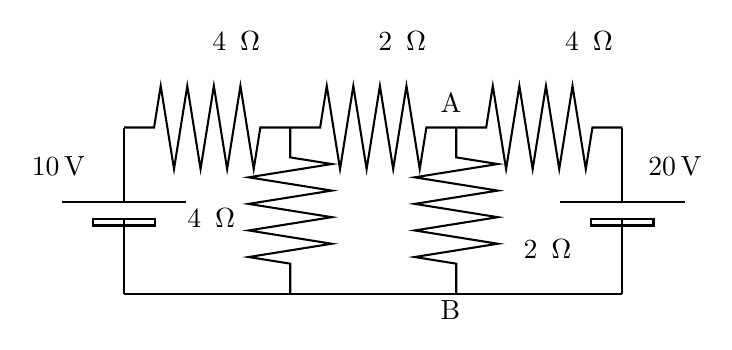
\begin{tikzpicture}[x=0.75pt,y=0.75pt,yscale=-1,xscale=1]
				%uncomment if require: \path (0,199); %set diagram left start at 0, and has height of 199
				%Shape: Resistor [id:dp1308381335020341] 
				\draw   (223,70) -- (223,84.4) -- (243,87.6) -- (203,94) -- (243,100.4) -- (203,106.8) -- (243,113.2) -- (203,119.6) -- (243,126) -- (203,132.4) -- (223,135.6) -- (223,150) ;
				%Shape: Resistor [id:dp43227316406655225] 
				\draw   (303,70) -- (303,84.4) -- (323,87.6) -- (283,94) -- (323,100.4) -- (283,106.8) -- (323,113.2) -- (283,119.6) -- (323,126) -- (283,132.4) -- (303,135.6) -- (303,150) ;
				%Shape: Resistor [id:dp8338029736541286] 
				\draw   (143,70) -- (157.4,70) -- (160.6,50) -- (167,90) -- (173.4,50) -- (179.8,90) -- (186.2,50) -- (192.6,90) -- (199,50) -- (205.4,90) -- (208.6,70) -- (223,70) ;
				%Shape: Resistor [id:dp47083902917006193] 
				\draw   (223,70) -- (237.4,70) -- (240.6,50) -- (247,90) -- (253.4,50) -- (259.8,90) -- (266.2,50) -- (272.6,90) -- (279,50) -- (285.4,90) -- (288.6,70) -- (303,70) ;
				%Shape: Resistor [id:dp1624776475468488] 
				\draw   (303,70) -- (317.4,70) -- (320.6,50) -- (327,90) -- (333.4,50) -- (339.8,90) -- (346.2,50) -- (352.6,90) -- (359,50) -- (365.4,90) -- (368.6,70) -- (383,70) ;
				%Shape: Battery [id:dp9409587079276216] 
				\draw   (143,150) -- (143,114) (113,106) -- (173,106) (143,106) -- (143,70) (128,117.2) -- (128,114) -- (158,114) -- (158,117.2) -- (128,117.2) -- cycle ;
				%Shape: Battery [id:dp2765193856004551] 
				\draw   (383,150) -- (383,114) (353,106) -- (413,106) (383,106) -- (383,70) (368,117.2) -- (368,114) -- (398,114) -- (398,117.2) -- (368,117.2) -- cycle ;
				%Straight Lines [id:da7366942904453511] 
				\draw    (143,150) -- (383,150) ;
				% Text Node
				\draw (184,22.4) node [anchor=north west][inner sep=0.75pt]    {$4\ {\Ohm}$};
				% Text Node
				\draw (264,22.4) node [anchor=north west][inner sep=0.75pt]    {$2\ {\Ohm}$};
				% Text Node
				\draw (354,22.4) node [anchor=north west][inner sep=0.75pt]    {$4\ {\Ohm}$};
				% Text Node
				\draw (172,107.4) node [anchor=north west][inner sep=0.75pt]    {$4\ {\Ohm}$};
				% Text Node
				\draw (334,122.4) node [anchor=north west][inner sep=0.75pt]    {$2\ {\Ohm}$};
				% Text Node
				\draw (294,52) node [anchor=north west][inner sep=0.75pt]   [align=left] {A};
				% Text Node
				\draw (97,82.4) node [anchor=north west][inner sep=0.75pt]    {$10\V$};
				% Text Node
				\draw (394,82.4) node [anchor=north west][inner sep=0.75pt]    {$20\V$};
				% Text Node
				\draw (294,152) node [anchor=north west][inner sep=0.75pt]   [align=left] {B};
			\end{tikzpicture}
		\end{figure}
	\end{eg}
	\begin{explanation}
		There are three meshes, let the currents be $I_1$, $I_2$ and $I_3$\footnote{from left mesh to right}.
		\[\begin{split}
			10-4I_1-4(I_1-I_2)&=0\\
			-2I_2-2(I_2-I_3)-4(I_2-I_1)&=0\\
			-20-2(I_3-I_2)-4I_3&=0
		\end{split}\]
		Thus,
		\[I_1=1.093\Amp\land I_2=-0.312\Amp\land I_3-3.437\Amp\]
		The current in AB is, $3.125$ from B to A.
	\end{explanation}
	\begin{eg}[Supermesh]
		Find the current in $5\Ohm$ resistance.
		\begin{figure}[H]
			\centering
			
			
			\tikzset{every picture/.style={line width=0.75pt}} %set default line width to 0.75pt        
			
			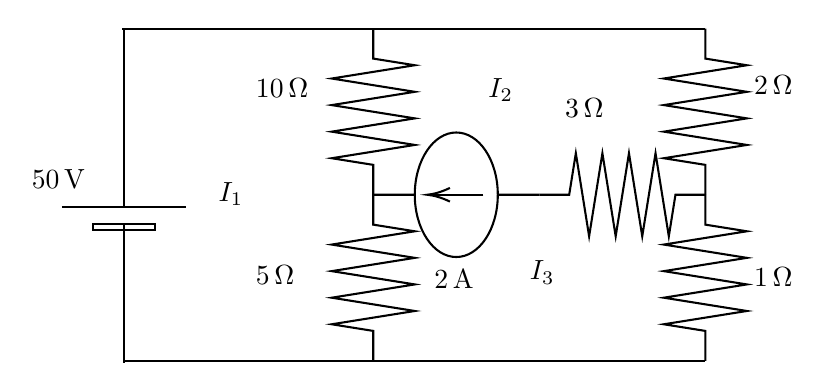
\begin{tikzpicture}[x=0.75pt,y=0.75pt,yscale=-1,xscale=1]
				%uncomment if require: \path (0,257); %set diagram left start at 0, and has height of 257
				
				%Shape: Battery [id:dp628303888513664] 
				\draw   (127,160) -- (127,124) (97,116) -- (157,116) (127,116) -- (127,80) (112,127.2) -- (112,124) -- (142,124) -- (142,127.2) -- (112,127.2) -- cycle ;
				
				%Shape: Resistor [id:dp6514308622236673] 
				\draw   (247,30) -- (247,44.4) -- (267,47.6) -- (227,54) -- (267,60.4) -- (227,66.8) -- (267,73.2) -- (227,79.6) -- (267,86) -- (227,92.4) -- (247,95.6) -- (247,110) ;
				%Shape: Resistor [id:dp8658086948445278] 
				\draw   (247,110) -- (247,124.4) -- (267,127.6) -- (227,134) -- (267,140.4) -- (227,146.8) -- (267,153.2) -- (227,159.6) -- (267,166) -- (227,172.4) -- (247,175.6) -- (247,190) ;
				
				%Shape: Resistor [id:dp008066100412755128] 
				\draw   (407,30) -- (407,44.4) -- (427,47.6) -- (387,54) -- (427,60.4) -- (387,66.8) -- (427,73.2) -- (387,79.6) -- (427,86) -- (387,92.4) -- (407,95.6) -- (407,110) ;
				%Shape: Resistor [id:dp5938017479280995] 
				\draw   (407,110) -- (407,124.4) -- (427,127.6) -- (387,134) -- (427,140.4) -- (387,146.8) -- (427,153.2) -- (387,159.6) -- (427,166) -- (387,172.4) -- (407,175.6) -- (407,190) ;
				
				%Shape: Resistor [id:dp592373074203639] 
				\draw   (327,110) -- (341.4,110) -- (344.6,90) -- (351,130) -- (357.4,90) -- (363.8,130) -- (370.2,90) -- (376.6,130) -- (383,90) -- (389.4,130) -- (392.6,110) -- (407,110) ;
				
				%Shape: Output [id:dp5978458432854965] 
				\draw   (267,110) .. controls (267,93.43) and (275.95,80) .. (287,80) .. controls (298.05,80) and (307,93.43) .. (307,110) .. controls (307,126.57) and (298.05,140) .. (287,140) .. controls (275.95,140) and (267,126.57) .. (267,110) -- cycle (247,110) -- (267,110) (327,110) -- (307,110) ;
				%Straight Lines [id:da7978659666363379] 
				\draw    (300,110) -- (275,110) ;
				\draw [shift={(273,110)}, rotate = 360] [color={rgb, 255:red, 0; green, 0; blue, 0 }  ][line width=0.75]    (10.93,-3.29) .. controls (6.95,-1.4) and (3.31,-0.3) .. (0,0) .. controls (3.31,0.3) and (6.95,1.4) .. (10.93,3.29)   ;
				%Straight Lines [id:da8911292086496967] 
				\draw    (247,30) -- (407,30) ;
				%Straight Lines [id:da3970728392462133] 
				\draw    (247,190) -- (407,190) ;
				%Straight Lines [id:da5819302056761924] 
				\draw    (126,30) -- (247,30) ;
				%Straight Lines [id:da6928824967599594] 
				\draw    (127,190) -- (247,190) ;
				%Straight Lines [id:da3286763229829708] 
				\draw    (127,30) -- (127,80) ;
				%Straight Lines [id:da5410055548378867] 
				\draw    (127,160) -- (127,191) ;
				
				% Text Node
				\draw (81,96.4) node [anchor=north west][inner sep=0.75pt]    {$50\V$};
				% Text Node
				\draw (189,52.4) node [anchor=north west][inner sep=0.75pt]    {$10\Ohm$};
				% Text Node
				\draw (429,51) node [anchor=north west][inner sep=0.75pt]    {$2\Ohm$};
				% Text Node
				\draw (189,142.4) node [anchor=north west][inner sep=0.75pt]    {$5\Ohm$};
				% Text Node
				\draw (429,143.8) node [anchor=north west][inner sep=0.75pt]    {$1\Ohm$};
				% Text Node
				\draw (338,62.4) node [anchor=north west][inner sep=0.75pt]    {$3\Ohm$};
				% Text Node
				\draw (275,144.4) node [anchor=north west][inner sep=0.75pt]    {$2\Amp$};
				% Text Node
				\draw (171,102.4) node [anchor=north west][inner sep=0.75pt]    {$I_{1}$};
				% Text Node
				\draw (301,52.4) node [anchor=north west][inner sep=0.75pt]    {$I_{2}$};
				% Text Node
				\draw (321,140.4) node [anchor=north west][inner sep=0.75pt]    {$I_{3}$};
			\end{tikzpicture}
		\end{figure}
	\end{eg}
	\begin{explanation}
		The current in each mesh is clockwise.
		\[\begin{split}
			-10(I_1-I_2)-5(I_1-I_3)+50&=0
		\end{split}\]
		The meshes with $I_2$ and $I_3$ constitute a supermesh, thus the equation for the supermesh is $I_2-I_3=2$, now, we neglect the $2\Amp$ and $3\Ohm$ and apply KVL to supermesh,
		\[-10(I_2-I_1)-2I_2-I_3-5(I_3-I_2)=0\]
		Thus, we get,
		\[I_1=20\Amp \land I_2=17.33\Amp \land 15.33\Amp\]
		The current in $5\Ohm$ resistance is $I_1-I_3=4.67\Amp$.
	\end{explanation}
	\subsection{Kirchhoff's Current Law}
	The algebraic sum of all the currents meeting at a point or a junction will be zero.
	\[\sum I=0\]
\end{document}